\providecommand{\main}{..}

\documentclass[\main/main]{subfiles}

\setcounter{chapter}{4}

\begin{document}

\tableofcontents

\chapter{Exploration in MDPs}



\section{Introduction}

One of the key challenges of reinforcement learning is the \gls{exploration-exploitation tradeoff}. Should we \emph{exploit} actions we know will give high reward, or should we \emph{explore} different actions to discover potentially better strategies?
An algorithm that doesn't explore effectively might easily \emph{overfit} to certain areas of the state space, and fail to generalize once they enter a region they haven't yet seen.
The algorithms we saw in the chapter on fitted DP \eqref{ch:fitted_dp} suffer from this issue.

In the \acrlong{mab} chapter \eqref{ch:mab}, where the state never changes so all we care about are the actions, we saw algorithms like UCB \ref{df:ucb} and Thompson sampling \ref{df:thompson_sampling} that incentivize the learner to explore arms that it is uncertain about.
In this chapter, we will see how to generalize these ideas to the MDP setting.

\begin{definition}{Per-episode regret}{per_episode_regret}
    To quantify the performance of a learning algorithm, we will consider its per-episode regret over $T$ timesteps/episodes:
    \[
        \text{Regret}_T = \E\left[ \sum_{t=0}^{T-1} \Vopt_0(s_0) - V^{\pi^t}_0(s_0) \right]
    \]
    where $\pi^t$ is the policy generated by the algorithm at the $t$th iteration.
\end{definition}

\subsection{Sparse reward}

Exploration is especially crucial in \textbf{sparse reward} problems where reward doesn't come until after many steps,
and algorithms which do not \emph{systematically} explore new states may fail to learn anything meaningful (within a reasonable amount of time).

For example, policy gradient algorithms require the gradient to be nonzero in order to learn. If we never observe any reward, the gradient will always be zero, and the policy will never change or improve.

\begin{example}{Sparse Reward MDP}{sparse_reward_mdp}
    Here's a simple example of an MDP with sparse reward:

    \begin{center}
        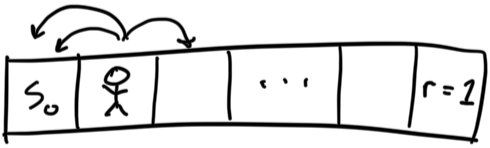
\includegraphics{assets/sparse_reward_mdp}
    \end{center}

    There are $|\S|$ states.
    The agent starts in the leftmost state.
    In every state, there are three possible actions, two of which move the agent left and one which moves the agent right. The reward function assigns $r=1$ to the rightmost cell.
\end{example}


\subsection{Exploration in deterministic MDPs}

Let us address the exploration problem in a \emph{deterministic} MDP where taking action $a$ in state $s$ always leads to the state $P(s, a) \in \S$.
In this simple setting, there will be no ``automatic'' exploration due to randomness, so our strategy must actively explore new states.
One simple strategy is to visit every possible state-action pair to learn the entire MDP.
Then, once the MDP is known, we can use DP to solve for the optimal policy.
(This should remind you of the \acrlong{etc} algorithm for \acrshortpl{mab} \eqref{df:etc}.)

\begin{definition}{Explore-then-exploit (for deterministic MDPs)}{explore_then_exploit}
    We'll keep a set $K$ of all the $(s, a, r, s')$ pairs we've observed.
    Each episode, we'll choose an unseen state-action pair for which the reward and the next state are unknown, and take the shortest path there.
    We assume that every state can be reached from the initial state within a single episode.

    \begin{algorithmic}
        \State $K \gets \emptyset$
        \While{$\exists (s, a)$ not explored (i.e. there is no $(s, a, r, s') \in K$)}
        \State Using our known transitions $K$, compute the shortest path $\tilde \pi$ to $(s, a)$
        \State Execute $\tilde \pi$ to visit $(s, a)$ and observe $r = r(s, a), s' = P(s, a)$
        \State $K \gets K \cup \{ (s, a, r, s') \}$
        \EndWhile
        \State Compute the optimal policy $\pi^\star$ in the MDP $K$ (e.g. using policy iteration).
        \State \Return $\pi^\star$.
    \end{algorithmic}

    The shortest path computation can be implemented using DP. We leave this as an exercise.
\end{definition}

\begin{theorem}{Performance of explore-then-exploit}{explore_then_exploit_performance}
    As long as every state can be reached from $s_0$ within a single episode, i.e. $|\S| \le \hor$, this will eventually be able to explore all $|\S| |\A|$ state-action pairs, adding one new transition per episode.
    We know it will take at most $|\S| |\A|$ iterations to explore the entire MDP, after which $\pi^t = \pi^\star$, incurring no additional regret.
    For each $\pi^t$ up until then, corresponding to the shortest-path policies $\tilde \pi$, the value of policy $\pi^t$ will differ from that of $\pi^\star$ by at most $\hor$, since the policies will differ by at most $1$ reward at each timestep.
    So,
    \[
        \sum_{t=0}^{T-1} \Vopt_0 - V_0^{\pi^t} \le |\S||\A| \hor.
    \]
    (Note that this MDP and algorithm are deterministic, so the regret is not random.)
\end{theorem}



\section{Treating an unknown MDP as a MAB}
\label{sec:mdp_mab}

We also explored the exploration-exploitation tradeoff in the chapter on \acrlong{mab} \eqref{ch:1_bandits}.
Recall tthat in the MAB setting, we have $K$ arms, each of which has an unknown reward distribution,
and we want to learn which of the arms is \emph{optimal}, i.e. has the highest mean reward.

One algorithm that struck a good balance between exploration and exploitation was the \textbf{upper confidence bound} algorithm \eqref{df:ucb}: For each arm, we construct a \emph{confidence interval} for its true mean award, and then choose the arm with the highest upper confidence bound. In summary,
\[k_{t+1} \gets \argmax_{k \in [K]} \frac{R^{k}_t}{N^{k}_t} + \sqrt{\frac{\ln(2t/\delta)}{2 N^{k}_t}}\]
where $N_t^k$ indicates the number of times arm $k$ has been pulled up until time $t$,
$R_t^k$ indicates the total reward obtained by pulling arm $k$ up until time $t$,
and $\delta > 0$ controls the width of the confidence interval.
How might we extend UCB to the MDP case?

Let us formally describe an unknown MDP as an MAB problem.
In an unknown MDP, we want to learn which \emph{policy} is optimal. So if we want to apply MAB techniques to solving an MDP, it makes sense to think of \emph{arms} as \emph{policies}.
There are $K = (|\A|^{|\S|})^\hor$ deterministic policies in a finite MDP.
Then, ``pulling'' arm $\pi$ corresponds to using $\pi$ to act through a trajectory in the MDP, and observing the total reward.

\begin{exercise}
    Which quantity that we have seen so far equals the mean reward from arm $\pi$?
\end{exercise}

Recall that UCB incurs regret $\tilde{O}(\sqrt{TK})$, where $T$ is the number of pulls and $K$ is the number of arms.
So in the MDP-as-MAB problem, using UCB for $T$ episodes would achieve regret
\begin{equation}
    \tilde{O}(\sqrt{|\A|^{|\S|\hor} T}).
    \label{eq:mdp_as_mab}
\end{equation}
This scales \emph{exponentially} in $|\S|$ and $\hor$, which quickly becomes intractable.
Notably, this method doesn't consider the information that we gain across different policies. We can illustrate this with the following example:

\begin{example}{Treating an MDP as a MAB is ineffective}{ineffective_mdp}
    Consider a ``coin MDP'' with two states ``heads'' and ``tails'', two actions ``Y'' and ``N'', and a time horizon of $\hor=2$.
    The state transition flips the coin, and doesn't depend on the action.
    The reward only depends on the action: Taking action Y gives reward $1$, and taking action N gives reward $0$.

    Suppose we collect data from the two constant policies $\pi_{\text{Y}}(s) = \text{Y}$ and $\pi_{\text{N}}(s) = \text{N}$.
    Now we want to learn about the policy $\tilde{\pi}$ that takes action Y and then N.
    Do we need to collect data from $\tilde{\pi}$ to evaluate it?
    No: Since the reward only depends on the action, we can infer its value from our data on the policies $\pi_{\text{Y}}$ and $\pi_{\text{N}}$.
    However, if we treat the MDP as a bandit in which $\tilde{\pi}$ is a new, unknown arm, we ignore the known correlation between the action and the reward.
\end{example}



\section{UCB-VI}

The approach above is inefficient: We shouldn't need to consider all $|\A|^{|\S| H}$ deterministic policies to achieve low regret.
Rather, all we need to describe the optimal policy is $\Qopt$, which has $H |\S||\A|$ entries to be learned.
Can we borrow ideas from UCB to reduce the regret to this order (i.e. polynomial in $|\S|$, $|\A|$, and $H$)?

One way to frame the UCB algorithm is that, when choosing arms, we optimize over a \emph{proxy reward} that is the sum of the estimated mean reward and an exploration term.
In the \textbf{UCB-VI} algorithm, we will extend this idea to the case of an unknown MDP $\mathcal{M}^{?}$ by modelling a proxy MDP $\tilde{\mathcal{M}}$ with a reward function that encourages exploration. Then, we will use DP to solve for the optimal policy in $\tilde{\mathcal{M}}$.

\textbf{Assumptions:} For simplicity, here we assume the reward function of $\mathcal{M}^{?}$ is known, so we only need to model the state transitions, though the rewards can be modelled similarly. We will also consider the more general case of a \textbf{time-varying} MDP, where the transition and reward functions can change over time. We take the convention that $P_\hi$ is the distribution of $s_{h+1} \mid s_{h}, a_{h}$ and $r_\hi$ is applied to $s_\hi, a_\hi$.

At a high level, the UCB-VI algorithm can be described as follows:

\begin{enumerate}
    \item \textbf{Modelling:} Use previous data to model the transitions $\hat{P}_0, \dots, \hat{P}_{H-1}$.
    \item \textbf{Reward bonus:} Design a reward bonus $b_\hi(s, a) \in \R$ to encourage exploration, analogous to the UCB term.
    \item \textbf{Optimistic planning:} Use DP to compute the optimal policy $\hat \pi_\hi(s)$ in the modelled MDP \[ \tilde{\mathcal{M}} = (\S, \A, \{ \hat{P}_\hi \}_{h \in [H]}, \{ r_\hi + b_\hi \}_{h \in [H]}, H). \]
    \item \textbf{Execution:} Use $\hat \pi_\hi(s)$ to collect a new trajectory, and repeat.
\end{enumerate}

We detail each of these steps below. The full definition follows in \eqref{df:ucb_vi}.


\subsection{Modelling the transitions}

% Let $\mathcal{D}_\hi^t$ denote the dataset of transitions collected at timestep $h$ from the first $t$ trajectories. That is, $\mathcal{D}_\hi^t = \{ s_\hi^i, a_\hi^i, s_{h+1}^i \}_{i \in [t]}$.

We seek to approximate $P_\hi(s_{h+1} \mid s_\hi, a_\hi) = \frac{\P(s_\hi, a_\hi, s_{h+1})}{\P(s_\hi, a_\hi)}$. We can estimate these using their sample probabilities from the dataset. That is, define
\begin{align*}
    N_\hi^t(s, a, s') & := \sum_{i=0}^{t-1} \ind{ (s_\hi^i, a_\hi^i, s_{h+1}^i) = (s, a, s') } \\
    N_\hi^t(s, a)     & := \sum_{i=0}^{t-1} \ind{ (s_\hi^i, a_\hi^i) = (s, a) }                \\
\end{align*}
Then we can model
\[
    \hat{P}_\hi^t(s' \mid s, a) = \frac{N_\hi^t(s, a, s')}{N_\hi^t(s, a)}.
\]
\begin{remark}
    Note that this is also a fairly naive, nonparametric estimator that doesn't assume any underlying structure of the MDP. We'll see how to incorporate assumptions about the MDP in the following section.
\end{remark}


\subsection{Reward bonus}

To motivate the reward bonus term $b_\hi^t(s, a)$, recall how we designed the reward bonus term for UCB:
\begin{enumerate}
    \item  We used Hoeffding's inequality to bound, with high probability, how far the sample mean $\hat \mu_t^k$ deviated from the true mean $\mu^k$.
    \item By inverting this inequality, we obtained a $(1-\delta)$-confidence interval for the true mean,
          centered at our estimate.
    \item To make this bound \emph{uniform} across all timesteps $t \in [T]$,
          we applied the union bound and multiplied $\delta$ by a factor of $T$.
\end{enumerate}

We'd like to do the same for UCB-VI, and construct the bonus term such that $\Vopt_\hi(s) \le \hat{V}_\hi^t(s)$ with high probability.
However, our construction will be more complex than the MAB case, since $\hat{V}_\hi^t(s)$ depends on the bonus $b_\hi^t(s, a)$ implicitly via DP.
We claim that the bonus term that gives the proper bound is
\begin{equation}
    b_\hi^t(s, a) = 2 H \sqrt{\frac{\log( |\S||\A|H T/\delta )}{N_\hi^t(s, a)}}.
    \label{eq:ucb_vi_bonus}
\end{equation}
We will only provide a heuristic sketch of the proof; see \cite[Section 7.3]{agarwal_reinforcement_2022} for a full proof.

\begin{derivation}{UCB-VI reward bonus construction}{ucb_vi_bonus}
    We aim to show that, with high probability, \[
        V_\hi^\star(s) \le \hat{V}_\hi^t(s) \quad \forall t \in [T], h \in [H], s \in \S.
    \]
    We'll do this by bounding the error incurred at each step of DP. Recall that DP solves for $\hat{V}_\hi^t(s)$ recursively as follows:
    \[
        \hat{V}_\hi^t(s) = \max_{a \in \A} \left[ \tilde r^t_\hi(s, a) + \E_{s' \sim \hat{P}_\hi^t(\cdot \mid s, a)} \left[ \hat{V}_{h+1}^t(s') \right] \right]
    \]
    where $\tilde r^t_\hi(s, a) = r_\hi(s, a) + b_\hi^t(s, a)$ is the reward function of our modelled MDP $\tilde{\mathcal{M}}^t$. On the other hand, we know that $\Vopt$ must satisfy
    \[
        \Vopt_\hi(s) = \max_{a \in \A} \left[ \tilde r^t_\hi(s, a) + \E_{s' \sim P^?_\hi(\cdot \mid s, a)} [\Vopt_{\hi+1}(s')] \right]
    \]
    so it suffices to bound the difference between the two inner expectations.
    There are two sources of error:
    \begin{enumerate}
        \item The value functions $\hat{V}^t_{h+1}$ v.s. $\Vopt_{h+1}$
        \item The transition probabilities $\hat{P}_\hi^t$ v.s. $P^?_\hi$.
    \end{enumerate}
    We can bound these individually, and then combine them by the triangle inequality.
    For the former, we can simply bound the difference by $H$, assuming that the rewards are within $[0, 1]$.
    Now, all that is left is to bound the error from the transition probabilities:
    \begin{equation}
        \text{error} = \left| \E_{s' \sim \hat{P}_\hi^t(\cdot \mid s, a)} \left[ \Vopt_{h+1}(s') \right] - \E_{s' \sim P^?_\hi(\cdot \mid s, a)} \left[ \Vopt_{h+1}(s') \right]. \right|
        \label{eq:err}
    \end{equation}

    Let us bound this term for a fixed $s, a, h, t$. (Later we can make this uniform across $s, a, h, t$ using the union bound.)
    Note that expanding out the definition of $\hat{P}_\hi^t$ gives
    \begin{align*}
        \E_{s' \sim \hat{P}_\hi^t(\cdot \mid s, a)} \left[ \Vopt_{h+1}(s') \right] & = \sum_{s' \in \S} \frac{N^t_\hi(s, a, s')}{N^t_\hi(s, a)} \Vopt_{h+1}(s')                                                     \\
                                                                                   & = \frac{1}{N^t_\hi(s, a)} \sum_{i=0}^{t-1} \sum_{s' \in \S} \ind{ (s_\hi^i, a_\hi^i, s_{h+1}^i) = (s, a, s') } \Vopt_{h+1}(s') \\
                                                                                   & = \frac{1}{N^t_\hi(s, a)} \sum_{i=0}^{t-1} \underbrace{\ind{ (s_\hi^i, a_\hi^i) = (s, a) } \Vopt_{h+1}(s_{h+1}^i)}_{X^i}
    \end{align*}
    since the terms where $s' \neq s_{h+1}^i$ vanish.

    Now, in order to apply Hoeffding's inequality, we would like to express the second term in \eqref{eq:err} as a sum over $t$ random variables as well. We will do this by redundantly averaging over all desired trajectories (i.e. where we visit state $s$ and action $a$ at time $h$):
    \begin{align*}
        \E_{s' \sim P^?_\hi(\cdot \mid s, a)} \left[ \Vopt_{h+1}(s') \right]
         & = \sum_{s' \in \S} P^?_\hi(s' \mid s, a) \Vopt_{h+1}(s')                                                                              \\
         & = \sum_{s' \in \S} \frac{1}{N^t_\hi(s, a)} \sum_{i=0}^{t-1} \ind{ (s_\hi^i, a_\hi^i) = (s, a) } P^?_\hi(s' \mid s, a) \Vopt_{h+1}(s') \\
         & = \frac{1}{N^t_\hi(s, a)} \sum_{i=0}^{t-1} \E_{s_{h+1}^i \sim P^?_{h}(\cdot \mid s_\hi^i, a_\hi^i)} X^i.
    \end{align*}
    Now we can apply Hoeffding's inequality to $X^i - \E_{s_{h+1}^i \sim P^?_{h}(\cdot \mid s_\hi^i, a_\hi^i)} X^i$, which is bounded by $\hor$, to obtain that, with probability at least $1-\delta$,
    \[
        \text{error} = \left| \frac{1}{N^t_\hi(s, a)} \sum_{i=0}^{t-1} \left(X^i - \E_{s_{h+1}^i \sim P^?_{h}(\cdot \mid s_\hi^i, a_\hi^i)} X^i \right) \right| \le 2 H \sqrt{\frac{\ln(1/\delta)}{N_\hi^t(s, a)}}.
    \]
    Applying a union bound over all $s \in \S, a \in \A, t \in [T], h \in [H]$ gives the $b_\hi^t(s, a)$ term above.
\end{derivation}


\subsection{Definition}

Putting these parts together, we can define the algorithm as follows:

\begin{definition}{UCB-VI}{ucb_vi}
    \begin{algorithmic}
        \For{$t \in [T]$}
        \State
        $N_\hi(s, a, s') \gets \sum_{i=0}^{t-1} \ind{ (s_\hi^i, a_\hi^i, s_{h+1}^i) = (s, a, s') }$
        \State $N_\hi(s, a) \gets \sum_{i=0}^{t-1} \ind{ (s_\hi^i, a_\hi^i) = (s, a) }$
        \State $\hat P_\hi \gets \frac{N_\hi(s, a, s')}{N_\hi(s, a)}$
        \Comment{Modelled transitions}
        \State $b_\hi(s, a) \gets 2 H \sqrt{\frac{\log( |\S||\A|H T/\delta )}{N_\hi(s, a)}}$
        \Comment{Reward bonus}
        \State $\tilde{\mathcal{M}} \gets (\S, \A, \{ \hat{P}_\hi \}_{h \in [H-1]}, \{ r_\hi + b_\hi \}_{h \in [H-1]}, H)$
        \Comment{Modelled MDP}
        \State $\hat \pi \gets \text{VI}(\tilde{\mathcal{M}})$
        \Comment{Planning with exploration bonus}
        \State Use $\hat \pi_h(s)$ to collect a new trajectory $(s^t_\hi, a^t_\hi, s^t_{\hi+1})_{\hi \in [\hor]}$
        \EndFor
    \end{algorithmic}
\end{definition}

\subsection{Performance of UCB-VI}

How exactly does UCB-VI strike a good balance between exploration and exploitation? In UCB for MABs, the bonus exploration term is simple to interpret: It encourages the learner to take actions with a high exploration term.
Here, the policy depends on the bonus term indirectly: The policy is obtained by planning in an MDP where the bonus term is added to the reward function.
Note that the bonuses \emph{propagate backwards} in DP, effectively enabling the learner to \emph{plan to explore} unknown states.
This effect takes some further interpretation.

Recall we constructed $b^t_\hi$ so that, with high probability, $\Vopt_\hi(s) \le \hat{V}_\hi^t(s)$ and so \[
    \Vopt_\hi(s) - V^{\pi^t}_\hi(s) \le \hat{V}_\hi^t(s) - V^{\pi^t}_\hi(s).
\]
That is, the l.h.s. measures how suboptimal policy $\pi^t$ is in the true environment,
while the r.h.s. is the difference in the policy's value when acting in the modelled MDP $\tilde{\mathcal{M}}^t$ instead of the true one $\mathcal{M}^{?}$.

If the r.h.s. is \emph{small}, this implies that the l.h.s. difference is also small, i.e. that $\pi^t$ is \emph{exploiting} actions that are giving high reward.

If the r.h.s. is \emph{large}, then we have overestimated the value: $\pi^t$, the optimal policy of $\tilde{\mathcal{M}}^t$, does not perform well in the true environment $\mathcal{M}^{?}$. This indicates that one of the $b_h^t(s, a)$ terms must be large, or some $\hat P^t_\hi(\cdot \mid s, a)$ must be inaccurate, indicating a state-action pair with a low visit count $N^t_\hi(s, a)$ that the learner was encouraged to explore.

It turns out that UCB-VI achieves a per-episode regret of
\begin{theorem}{UCB-VI regret}{ucb_vi_regret}
    \[
        \E \left[ \sum_{t=0}^{T-1} \left(\Vopt_0(s_0) - V^{\pi^t}_0(s_0) \right) \right] = \tilde{O}(H^2 \sqrt{|\S| |\A| T})
    \]
\end{theorem}

Comparing this to the UCB regret bound $\tilde{O}(\sqrt{T K})$, where $K$ is the number of arms of the MAB, we see that we've reduced the number of effective arms from
$|\A|^{|\S|\hor}$ (in \eqref{eq:mdp_as_mab}) to $H^4 |\S||\A|$, which is indeed polynomial in $|\S|$, $|\A|$, and $H$, as desired.
This is also roughly the number of episodes it takes to achieve constant-order average regret:
\[
    \frac{1}{T} \E[\text{Regret}_T] = \tilde{O}\left(\sqrt{\frac{H^4 |\S||\A|}{T}}\right)
\]
Note that the time-dependent transition matrix has $H |\S|^2 |\A|$ entries.
Assuming $H \ll |\S|$, this shows that it's possible to achieve low regret, and achieve a near-optimal policy, while only understanding a $1/|\S|$ fraction of the world's dynamics.


\section{Linear MDPs}

A polynomial dependency on $|\S|$ and $|\A|$ is manageable when the state and action spaces are small.
But for large or continuous state and action spaces, even this polynomial factor will become intractable.
Can we find algorithms that don't depend on $|\S|$ or $|\A|$ at all,
effectively reducing the dimensionality of the MDP?
In this section, we'll explore \textbf{linear MDPs}: an example of a \emph{parameterized} MDP where the rewards and state transitions depend only on some parameter space of dimension $d$ that is independent from $|\S|$ or $|\A|$.

\begin{definition}{Linear MDP}{linear_mdp}
    We assume that the transition probabilities and rewards are \emph{linear} in some feature vector $\phi(s, a) \in \R^d$:
    \begin{align*}
        P_\hi(s' \mid s, a) & = \phi(s, a)^\top \mu^\star_\hi(s') \\
        r_\hi(s, a)         & = \phi(s, a)^\top \theta_\hi^\star
    \end{align*}
    Note that we can also think of $P_\hi(\cdot \mid s, a) = \mu_\hi^\star$ as an $|\S| \times d$ matrix, and think of $\mu^\star_\hi(s')$ as indexing into the $s'$-th row of this matrix (treating it as a column vector). Thinking of $\Vopt_{\hi+1}$ as an $|\S|$-dimensional vector, this allows us to write \[ \E_{s' \sim P_\hi(\cdot \mid s, a)}[\Vopt_{\hi+1}(s)] = (\mu^\star_\hi \phi(s, a))^\top \Vopt_{\hi+1}. \]
    The $\phi$ feature mapping can be designed to capture interactions between the state $s$ and action $a$.
    In this book, we'll assume that the feature map $\phi : \S \times \A \to \R^d$ and the reward function (described by $\theta_\hi^\star$) are known to the learner.
\end{definition}


\subsection{Planning in a linear MDP}

It turns out that $\Qopt_\hi$ is also linear with respect to this feature mapping.
We can prove this by simply computing it using DP.
We initialize $V_{H}^\star(s) = 0 \forall s$. Then we iterate:
\begin{align*}
    \Qopt_\hi(s, a)  & = r_\hi(s, a) + \E_{s' \sim P_\hi(\cdot \mid s, a)} [\Vopt_{h+1}(s')]                          \\
                     & = \phi(s, a)^\top \theta_\hi^\star + (\mu_\hi^\star \phi(s, a))^\top \Vopt_{h+1}               \\
                     & = \phi(s, a)^\top \underbrace{( \theta_\hi^\star + (\mu_\hi^\star)^\top  \Vopt_{h+1})}_{w_\hi} \\
    \Vopt_\hi(s)     & = \max_a \Qopt_\hi(s, a)                                                                       \\
    \pi^\star_\hi(s) & = \argmax_a \Qopt_\hi(s, a)
\end{align*}

\begin{exercise}
    Show that $Q^\pi_\hi$ is also linear with respect to $\phi(s, a)$ for any policy $\pi$.
\end{exercise}


\subsection{UCB-VI in a linear MDP}
\label{sec:lin_ucb_vi}

\subsubsection{Modelling the transitions}

This linear assumption on the MDP will also allow us to model the unknown dynamics $P^?_\hi(s' \mid s, a)$ with techniques from \textbf{supervised learning} (SL).
Recall that SL is useful for estimating conditional expectations by minimizing mean squared error.
We can rephrase the estimation of $P^?_\hi(s' \mid s, a)$ as a least-squares problem as follows:
Write $\delta_s$ to denote a one-hot vector in $\R^{|\S|}$, with a $1$ in the $s$-th entry and $0$ everywhere else.
Note that \[
    \E_{s' \sim P_h(\cdot \mid s, a)} [\delta_{s'}] = P_h(\cdot \mid s, a) = \mu_h^\star \phi(s, a).
\]
Furthermore, since the expectation here is linear with respect to $\phi(s, a)$, we can directly apply least-squares multi-target linear regression to construct the estimate
\[
    \hat \mu = \argmin_{\mu \in \R^{|\S| \times d}} \sum_{t=0}^{T-1} \|\mu \phi(s_h^i, a_h^i) - \delta_{s_{h+1}^i} \|_2^2.
\]
This has a well-known closed-form solution:
\begin{align*}
    \hat \mu^\top            & = (A_h^t)^{-1} \sum_{i=0}^{t-1} \phi(s_h^i, a_h^i) \delta_{s_{h+1}^i}^\top \\
    \text{where} \quad A_h^t & = \sum_{i=0}^{t-1} \phi(s_h^i, a_h^i) \phi(s_h^i, a_h^i)^\top + \lambda I
\end{align*}
where we include a $\lambda I$ term to ensure that the matrix $A^t_h$ is invertible. (This can also be derived by adding a $\lambda \|\mu\|_{\text{F}}^2$ regularization term to the objective.)
We can directly plug in this estimate into $\hat{P}^t_h(\cdot \mid s, a) = \hat \mu^t_h \phi(s, a)$.

\subsubsection{Reward bonus}

Now, to design the reward bonus, we can't apply Hoeffding anymore, since the terms no longer involve sample means of bounded random variables; Instead, we're incorporating information across different states and actions. Rather, we can construct an upper bound using \emph{Chebyshev's inequality} in the same way we did for the LinUCB algorithm in the MAB setting \ref{df:lin_ucb}:
\[
    b^t_\hi(s, a) = \beta \sqrt{\phi(s, a)^\top (A^t_h)^{-1} \phi(s, a)}, \quad \beta = \tilde O(d \hor).
\]
Note that this isn't explicitly inversely proportional to $N_h^t(s, a)$ as in the original UCB-VI bonus term \ref{eq:ucb_vi_bonus}. Rather, it is inversely proportional to the amount that the direction $\phi(s, a)$ has been explored in the history. That is, if $A_h^t$ has a large component in the direction $\phi(s, a)$, implying that this direction is well explored, then the bonus term will be small, and vice versa.

We can now plug in these transition estimates and reward bonuses into the UCB-VI algorithm \ref{df:ucb_vi}.

\subsubsection{Performance}

\begin{theorem}{LinUCB-VI regret}{lin_ucb_vi_regret}
    The LinUCB-VI algorithm achieves expected regret
    \[
        \E[\text{Regret}_T] = \E\left[\sum_{t=0}^{T-1} \Vopt_0(s_0) - V^{\pi^t}_0(s_0) \right] \le \tilde O(H^2 d^{1.5} \sqrt{T})
    \]
\end{theorem}

Comparing this to our bound for UCB-VI in an environment without this linear assumption, we see that we go from a sample complexity of $\tilde \Omega(H^4 |\S||\A|)$ to $\tilde \Omega(H^4 d^{3})$. This new sample complexity only depends on the feature dimension and not on the state or action space of the MDP!



\section{Summary}

In this chapter, we've explored how to explore in an unknown MDP.
\begin{itemize}
    \item  We first discussed the explore-then-exploit algorithm \eqref{df:explore_then_exploit}, a simple way to explore a deterministic MDP by visiting all state-action pairs.
    \item We then discussed how to treat an unknown MDP as a MAB \eqref{sec:mdp_mab}, and how this approach is inefficient since it doesn't make use of relationships between policies.
    \item We then introduced the UCB-VI algorithm \eqref{df:ucb_vi}, which models the unknown MDP by a proxy MDP with a reward bonus term that encourages exploration.
    \item Finally, assuming that the transitions and rewards are linear with respect to a feature transformation of the state and action, we introduced the LinUCB-VI algorithm \eqref{sec:lin_ucb_vi}, which has a sample complexity independent of the size of the state and action spaces.
\end{itemize}

\end{document}


